
    
Эта секция описывает все главные возможности, которые должны быть реализованы в системе для обработки входных данных и производства выходных данных. Здесь определены функциональные требования к системе, сгрупперованные по принадлежности к классу пользователей, и каждой дан уникальный идентификатор, чтобы ссылаться к нему в процессе разработки системы. Так же для функционального требования может быть указано одно или несколько дргих функциональных требований, от которых оно зависит. 

Так же для удобства восприятия атрибутов требований они представлены в сводной таблице \ref{tab:fr-summary}.

\subsection{Администратор}
\include{src/главы/введение/index}

\subsection{Редактор}
\include{src/главы/введение/index}

\subsection{Гость}
\include{src/главы/введение/index}


\begin{figure}
    \centering
    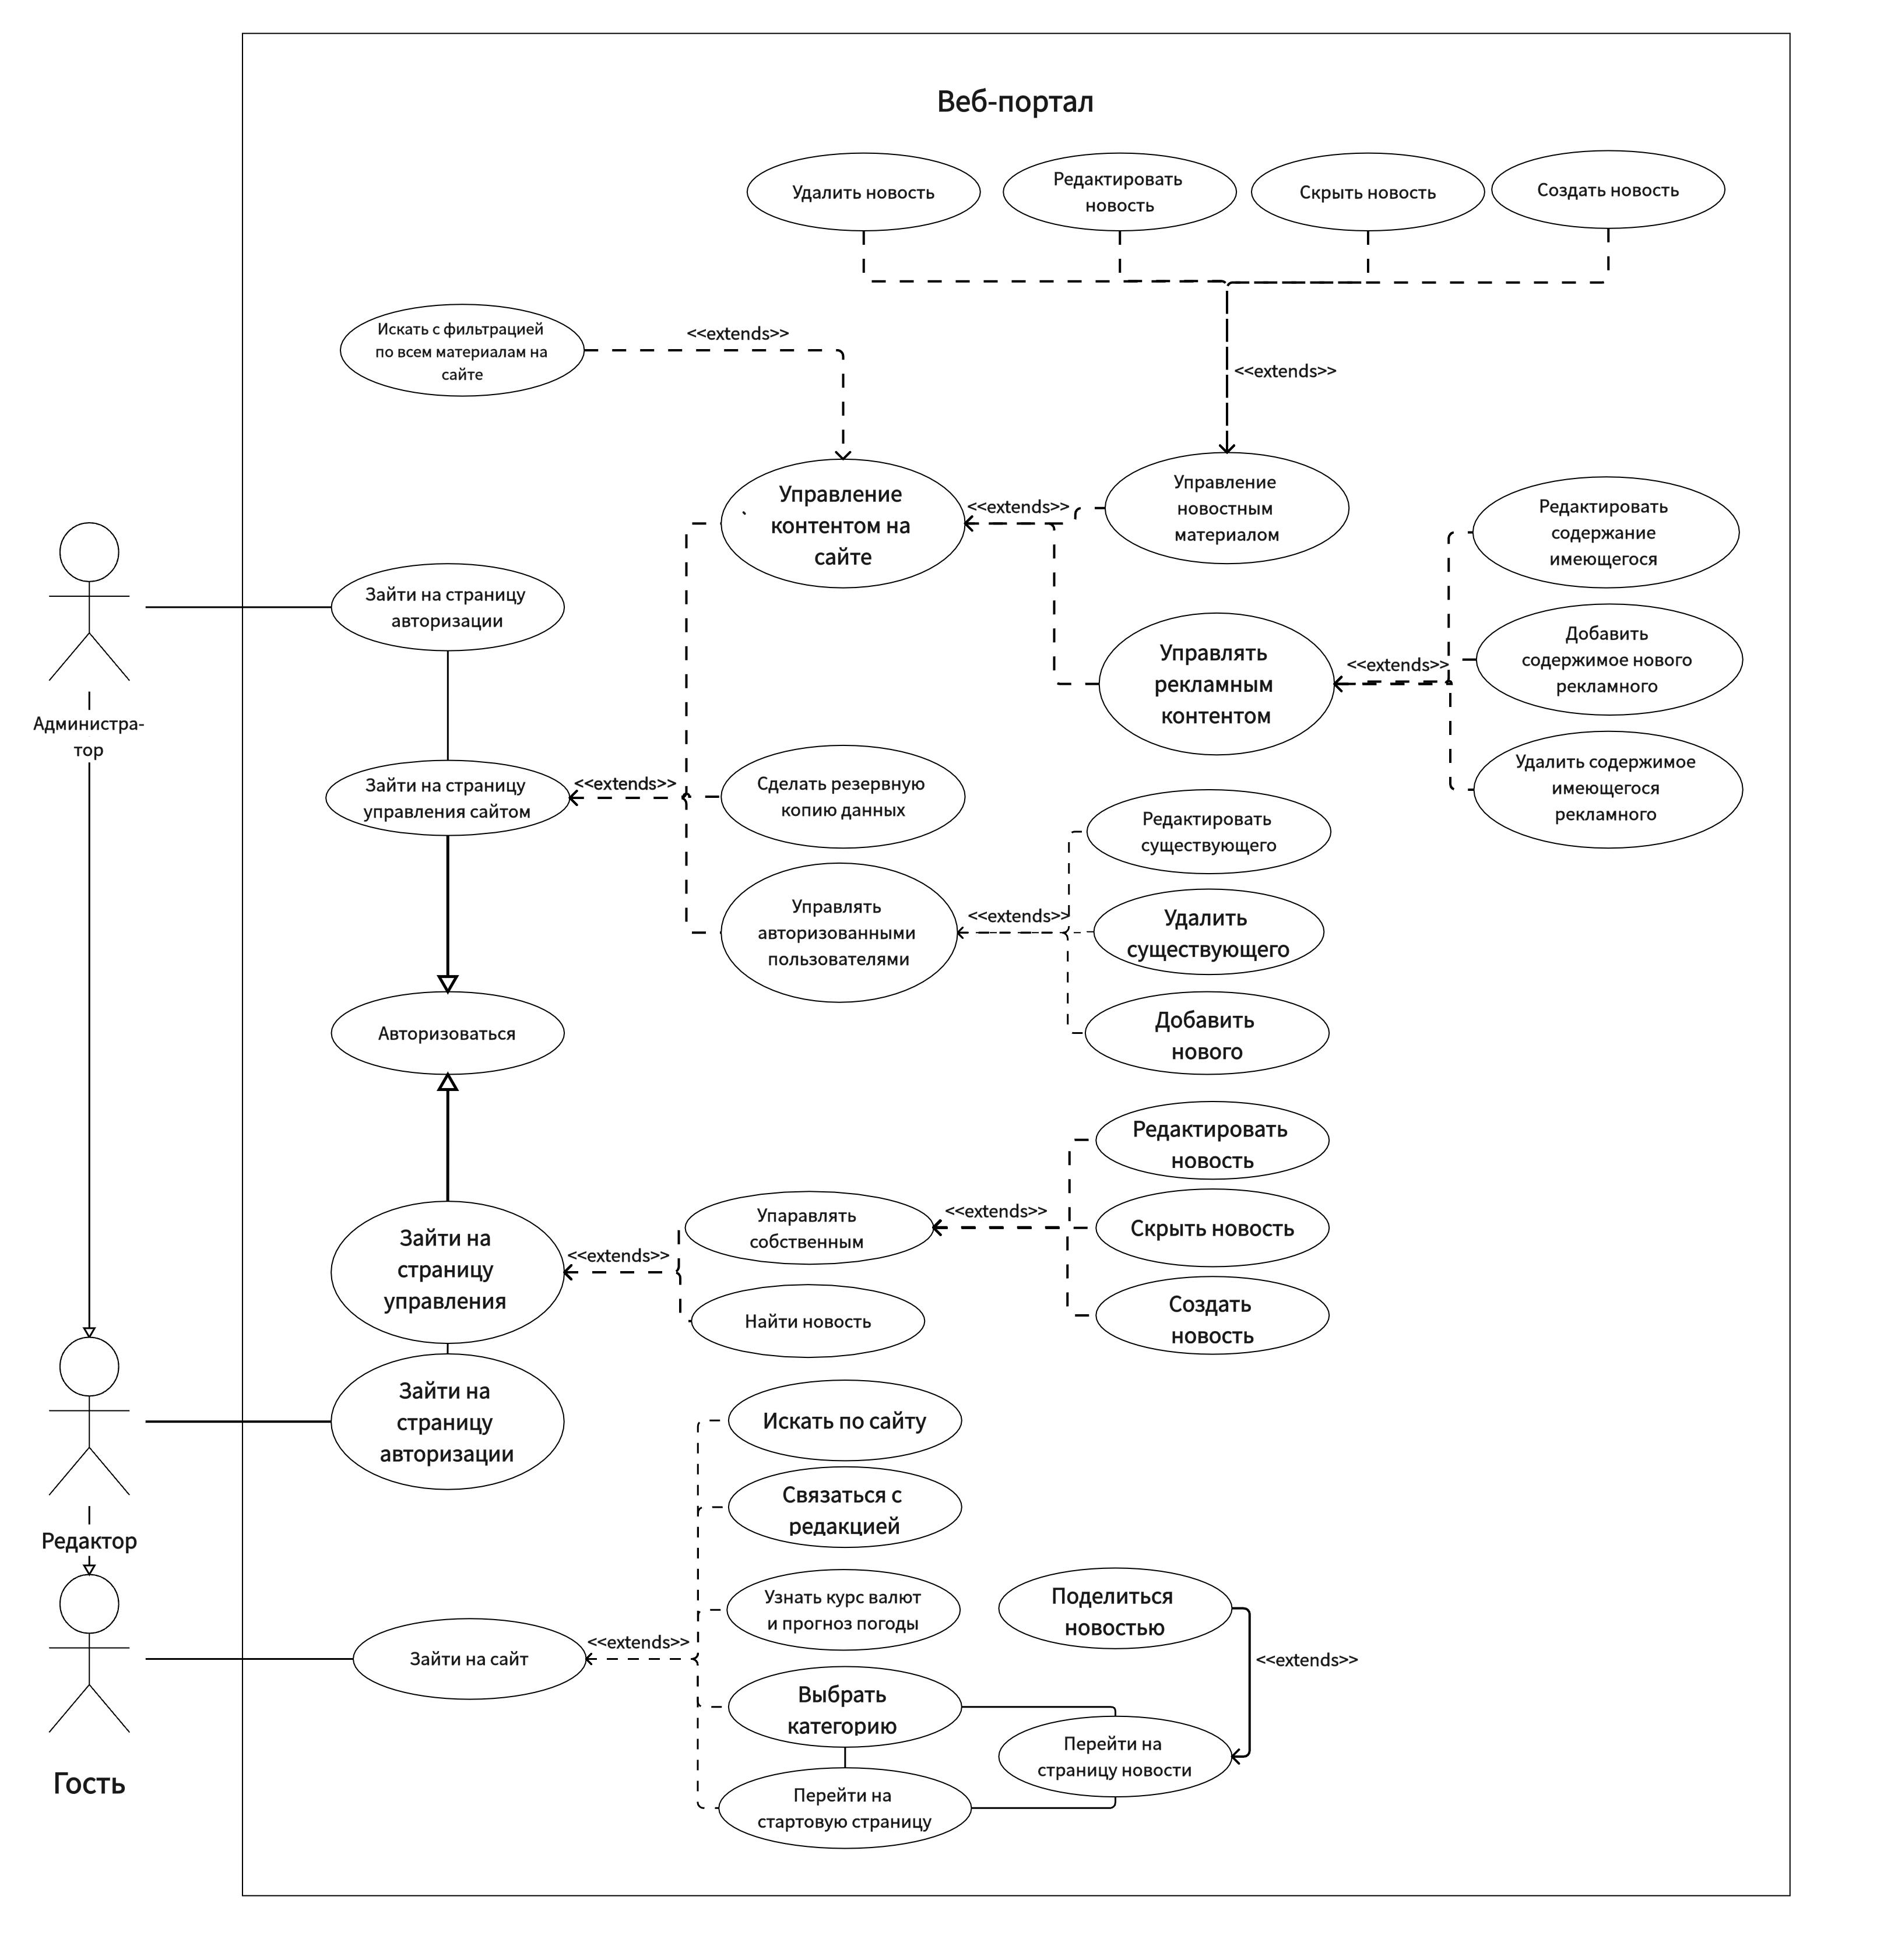
\includegraphics[width=0.85\paperwidth]{res/functional-requirements.png}
    \caption{Диаграмма способов использования}
    \label{fig:use-case-diagram}
\end{figure}

\begin{table}[]
    \centering
    \begin{tabular}{|l|l|l|l|l|}\hline
\textbf{ID}	&	\textbf{Название}	&	\textbf{Приоритет}	&	\textbf{Зависимости}	&	\textbf{Оценка времени,} 	\\	
	&		&		&		&	\textbf{чел.ч}	\\	\hline
FR1	&	Авторизация	&	высокий	&	-	&	20	\\	\hline
FR2	&	Управление пользователями	&	высокий	&	FR1	&	35	\\	\hline
FR3	&	Резервное копирование	&	высокий	&	FR1	&	30	\\	\hline
FR4	&	Управление новостным 	&	высокий	&	FR4	&	40	\\	
	&	материалом	&		&		&		\\	\hline
FR5	&	Поиск с фильтрацией	&	высокий	&	FR1	&	40	\\	
	&	по всем материалам	&		&		&		\\	\hline
FR6	&	Управление рекламным	&	высокий	&	FR1	&	40	\\	
	&	контентом	&		&		&		\\	\hline
FR7	&	Авторизация	&	высокий	&	FR2	&	20	\\	\hline
FR8	&	Управление новостями	&	высокий	&	FR4, FR7	&	30	\\	\hline
FR9	&	Управление новостями	&	высокий	&	FR2	&	20	\\	\hline
FR10	&	Просмотр новостей	&	высокий	&	-	&	60	\\	\hline
FR11	&	Прогноз погоды и курс валют	&	низкий	&	-	&	20	\\	\hline
FR12	&	Фильтрация новостей	&	высокий	&	FR5	&	20	\\	\hline
FR13	&	Поиск новостей	&	высокий	&	FR5, FR12	&	20	\\	\hline
FR14	&	Поделиться новостью	&	средний	&	FR10	&	20	\\	\hline
FR15	&	Связь с администрацией	&	средний	&	-	&	20	\\	\hline
    \end{tabular}
    \caption{Сводная таблица атрибутов функциональных требований.}
    \label{tab:fr-summary}
\end{table}

%%%%
%\textit{Functional requirements should define the fundamental actions that must take place in the software in
%accepting and processing the inputs and in processing and generating the These are generally listed
%as “shall” statements starting with Пе system shall...\\
%These include\\
%а) Validity checks оп the inputs\\
%Ь) Exact sequence of operations\\
%с) Responses to abnormal situations, including\\
%   1) Overfow\\
%   2) Communication facilities\\
%   З) Error handling and recovery\\
%d) Effect of parameters\\
%е) Relationship of outputs to inputs, inc1uding\\
%   1) Input/Output sequences\\
%   2) Formulas for input to output conversion
%\\
%It тау be appropriate to partition the functional requirements into subfunctions от subprocesses. This does
%not imply that the software design will also be partitioned that way.
%}
